\documentclass[../AP_Statistics.tex]{subfiles}

\begin{document}
	\chapter{Quantitative Data}
		Statistics is the science of collecting and analyzing data. \\
		A data set is a collection of data on several \textbf{individuals}. These individuals can be anything. \\
		Data provides values for \textbf{variables}, which describe some characteristic of an individual.
		A variable's \textbf{distribution} describes the frequency with which a variable takes on its possible values.
		\section{Graphically Displaying Distributions}
			Quantitative variables can either be \textbf{discrete}, having some countable set of possible values, or \textbf{continuous}, having an uncountably infinite set of possible values. \\
			\begin{center}
				\fbox{
				\begin{minipage}{17cm}
					The quantitative variable being described must always be defined, typically as a capital letter. An arbitrary particular value is denoted with a lowercase letter and a superscript is added to denote a defined value.	
				\end{minipage}}
					\comment{
					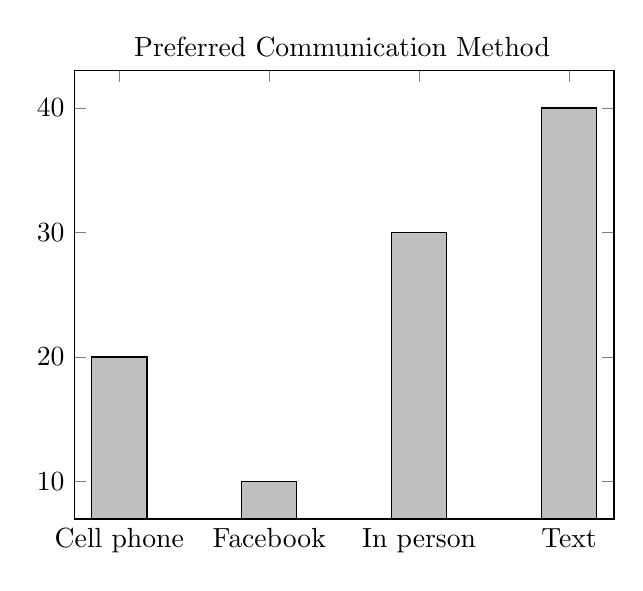
\begin{tikzpicture}
						\begin{axis}[bar width = 20pt, symbolic x coords = {Cell phone, Facebook, In person, Text}, xtick = data]
							\addplot[ybar, fill = lightgray] coordinates{(Cell phone, 20) (Facebook, 10) (In person, 30) (Text, 40)};
						\end{axis}
						\node at (3.4,6) {Preferred Communication Method};
					\end{tikzpicture}}
				\end{center}
				\textbf{Pie charts} show each category as some fraction of a circle that is bounded by two radii. The areas of each slice is proportional to the frequency.
		\section{Numerically Describing Distributions}
			The \textbf{mean} is the sum of each value (not necessarily unique) in the distribution divided by the total number of values. It is also referred to as the average or expected value of its variable. For a sample, it is denoted using a bar over the lowercase form of its variable ($X$ becoming $\bar{x}$).
			$$\bar{x} = \frac{\sum x_i}{n}$$
			The first, second, and third, \textbf{Quartiles}, denoted $Q_1, Q_2,$ and $Q_3$, are the values with 25\%, 50\%, and 75\% of the data below them respectively\footnote{This means that the probability of $X$ falling below each quartile is equal to its number multiplied by 25\%. $$P(X < Q_1) = 0.25 \hspace{1cm} P(X < Q_2) = 0.5 \hspace{1cm} P(X < Q_3) = 0.75$$}. The second quartile is the \textbf{median}, and is, along with the mean, a measure of center. \\
			The \textbf{range} is the difference between the highest and lowest values of a data set. \\
			The \textbf{interquartile range}, denoted $IQR$, is the difference between the values of the third and first quartiles \footnote{A box plot shows the interquartile range as the box and the median as the line within it.}. It therefore shows the "middle half" of the distribution.
			$$IQR = Q_3 - Q_1$$
			The \textbf{standard deviation} is the average distance from the mean for a value. It is denoted by $s$  with the subscript of its variable's lowercase form (for a sample). Along with the range and interquartile range, it is a measure of spread/variability.
			$$s_x = \sqrt{\frac{\sum (x_i - \bar{x})^2}{n - 1}}$$
			\begin{center}
				\fbox{
					\begin{minipage}{17cm}
						It is crucial to note that the mean and standard deviation are only to be used when there are no outliers, as they are sensitive.
					\end{minipage}}
			\end{center}
			The \textbf{variance} is the square of the standard deviation and is accordingly denoted by $s^2$ with the appropriate subscript. \\
			An \text{outlier} is any value that varies from the middle 50\% by over 1.5 multiplied by the interquartile range. \footnote{The values of $n, \sum x_i, \bar{x}, Q_1, Q_2, Q_3, $ range$, IQR, s_x, $ and $s_x^2$ are all calculable automatically given a data set. The data can be entered into $\texttt{L}n$ ($\texttt{Stat/EDIT/1}$), and $\texttt{1-Var Stats}$ ($\texttt{Stat/CALC/1}$) can be performed with $\texttt{L}n$ ($\texttt{ALPHA/}n$) as its parameter.}
	\chapter{Categorical Data}
		\textbf{Categorical variables} assign labels that place each individual into one of several groups, while \textbf{quantitative variables} provide values that describe or measure some characteristic. \\
		\section{Graphically Displaying Categorical Variables}
			A \textbf{frequency table} shows the number of individuals that have a certain value while a \textbf{relative frequency table} shows the percentage of all individuals in the data set that have that particular value. \\
			\textbf{Bar graphs} show each category as a bar, the height of which corresponds to its frequency. \\
\end{document}